\documentclass[12pt,a4paper]{article}
\usepackage[utf8]{inputenc}
\usepackage[T1]{fontenc}
\usepackage[vietnamese]{babel}
\usepackage{geometry}
\usepackage{graphicx}
\usepackage{float}
\usepackage{fancyhdr}
\usepackage{hyperref}
\usepackage{tikz}
\usetikzlibrary{shapes.geometric, arrows, positioning, shapes.multipart, fit, calc}
\usepackage{amsmath}
\usepackage{array}
\usepackage{longtable}
\usepackage{listings}
\usepackage{xcolor}
\usepackage{subcaption}
\usepackage{booktabs}
\usepackage{multirow}

% Code listing setup
\definecolor{codegreen}{rgb}{0,0.6,0}
\definecolor{codegray}{rgb}{0.5,0.5,0.5}
\definecolor{codepurple}{rgb}{0.58,0,0.82}
\definecolor{backcolour}{rgb}{0.95,0.95,0.92}

\lstdefinestyle{mystyle}{
    backgroundcolor=\color{backcolour},   
    commentstyle=\color{codegreen},
    keywordstyle=\color{magenta},
    numberstyle=\tiny\color{codegray},
    stringstyle=\color{codepurple},
    basicstyle=\ttfamily\footnotesize,
    breakatwhitespace=false,         
    breaklines=true,                 
    captionpos=b,                    
    keepspaces=true,                 
    numbers=left,                    
    numbersep=5pt,                  
    showspaces=false,                
    showstringspaces=false,
    showtabs=false,                  
    tabsize=2
}

\lstset{style=mystyle}

% Page setup
\geometry{left=3cm,right=2cm,top=2.5cm,bottom=2.5cm}
\pagestyle{fancy}
\fancyhf{}
\fancyhead[L]{\leftmark}
\fancyhead[R]{\thepage}
\renewcommand{\headrulewidth}{0.4pt}

% Title page setup
\title{\Huge\textbf{BÁO CÁO ĐỒ ÁN CHUYÊN NGÀNH}\\
\vspace{1cm}
\LARGE XÂY DỰNG PLATFORM HỌC TẬP\\
THUẬT TOÁN VÀ CẤU TRÚC DỮ LIỆU TƯƠNG TÁC\\
\vspace{0.5cm}
\large (DSA VISUALIZER PLATFORM)}

\author{
\textbf{SINH VIÊN:}\\
[Tên sinh viên] - [MSSV]\\
\vspace{0.5cm}\\
\textbf{GIẢNG VIÊN HƯỚNG DẪN:}\\
[Tên giảng viên]\\
\vspace{0.5cm}\\
\textbf{NGÀNH:} Công nghệ thông tin\\
\textbf{LỚP:} [Mã lớp]
}

\date{Thành phố Hồ Chí Minh, Tháng 12/2024}

\begin{document}

\maketitle
\newpage

\tableofcontents
\newpage

\section{Tóm tắt đồ án}

\subsection{Mục tiêu}
Đồ án này nhằm xây dựng một nền tảng học tập tương tác cho thuật toán và cấu trúc dữ liệu (DSA Visualizer Platform), giúp sinh viên và người học hiểu rõ hơn về các khái niệm phức tạp thông qua việc trực quan hóa và tương tác trực tiếp với các thuật toán.

\subsection{Phạm vi}
Platform cung cấp:
\begin{itemize}
    \item Trực quan hóa 24+ thuật toán khác nhau
    \item Hệ thống AI hỗ trợ học tập đa ngôn ngữ lập trình
    \item Cộng đồng học tập với forum và Q\&A
    \item Dashboard quản trị và phân tích dữ liệu
    \item Hệ thống xác thực và phân quyền người dùng
\end{itemize}

\subsection{Kết quả đạt được}
\begin{itemize}
    \item Xây dựng thành công platform đầy đủ tính năng
    \item Triển khai 24+ visualizer cho các thuật toán khác nhau
    \item Tích hợp AI (OpenAI GPT \& Google Gemini) hỗ trợ học tập
    \item Phát triển hệ thống cộng đồng và quản trị hoàn chình
    \item Đảm bảo tính responsive và accessibility
\end{itemize}

\section{Giới thiệu hệ thống}

\subsection{Giới thiệu đề tài}

Trong thời đại công nghệ 4.0, việc học tập các thuật toán và cấu trúc dữ liệu trở nên quan trọng hơn bao giờ hết. Tuy nhiên, nhiều sinh viên gặp khó khăn trong việc hiểu các khái niệm trừu tượng này chỉ thông qua lý thuyết. DSA Visualizer Platform được phát triển nhằm giải quyết vấn đề này bằng cách cung cấp một môi trường học tập tương tác, trực quan và hiện đại.

Platform này không chỉ đơn thuần là công cụ trực quan hóa mà còn là một hệ sinh thái học tập hoàn chỉnh với:
\begin{itemize}
    \item \textbf{Trực quan hóa tương tác}: Hơn 24 thuật toán được minh họa sinh động
    \item \textbf{AI Assistant}: Hỗ trợ học tập thông minh với 6 ngôn ngữ lập trình
    \item \textbf{Cộng đồng học tập}: Forum thảo luận và hệ thống Q\&A
    \item \textbf{Quản lý tiến độ}: Theo dõi quá trình học tập cá nhân
    \item \textbf{Đa nền tảng}: Hoạt động mượt mà trên mọi thiết bị
\end{itemize}

\subsection{Mục tiêu cụ thể}

\subsubsection{Mục tiêu chính}
\begin{enumerate}
    \item \textbf{Nâng cao hiệu quả học tập}: Giúp sinh viên hiểu thuật toán nhanh hơn 60\% thông qua trực quan hóa
    \item \textbf{Tạo môi trường tương tác}: Phát triển platform cho phép thực hành và thí nghiệm trực tiếp
    \item \textbf{Xây dựng cộng đồng}: Tạo không gian học tập collaborative với forum và Q\&A
    \item \textbf{Ứng dụng AI}: Tích hợp AI để cá nhân hóa trải nghiệm học tập
\end{enumerate}

\subsubsection{Mục tiêu kỹ thuật}
\begin{enumerate}
    \item \textbf{Hiệu năng cao}: Đảm bảo animation mượt mà với 60 FPS
    \item \textbf{Khả năng mở rộng}: Kiến trúc modular cho phép bổ sung thuật toán mới dễ dàng
    \item \textbf{Bảo mật}: Hệ thống xác thực multi-provider và phân quyền chi tiết
    \item \textbf{Responsive Design}: Hoạt động tối ưu trên desktop, tablet và mobile
\end{enumerate}

\subsection{Đối tượng sử dụng}

\begin{table}[H]
\centering
\caption{Phân loại người dùng hệ thống}
\begin{tabular}{|l|p{10cm}|}
\hline
\textbf{Nhóm người dùng} & \textbf{Mô tả và nhu cầu} \\
\hline
\textbf{Sinh viên} & Học tập các thuật toán cơ bản, thực hành coding, tham gia cộng đồng \\
\hline
\textbf{Giảng viên} & Sử dụng làm công cụ giảng dạy, tạo nội dung học tập, quản lý lớp học \\
\hline
\textbf{Lập trình viên} & Ôn tập thuật toán cho phỏng vấn, nghiên cứu thuật toán mới \\
\hline
\textbf{Người tự học} & Tìm hiểu thuật toán một cách tự động, có AI hỗ trợ \\
\hline
\textbf{Admin} & Quản lý hệ thống, theo dõi usage, xử lý feedback \\
\hline
\end{tabular}
\end{table}

\section{Phân tích yêu cầu}

\subsection{Yêu cầu chức năng}

\subsubsection{Hệ thống xác thực và phân quyền}
\begin{itemize}
    \item \textbf{RF-01}: Đăng ký/đăng nhập với email, Google, GitHub
    \item \textbf{RF-02}: Hệ thống phân quyền 4 cấp (Guest, User, Teacher, Admin)
    \item \textbf{RF-03}: Quản lý profile và theo dõi tiến độ học tập
    \item \textbf{RF-04}: Password reset và email verification
\end{itemize}

\subsubsection{Visualizer thuật toán}
\begin{itemize}
    \item \textbf{RF-05}: Trực quan hóa sorting algorithms (Quick, Merge, Heap, Radix, etc.)
    \item \textbf{RF-06}: Visualizer cho data structures (Binary Tree, AVL, Hash Table, etc.)
    \item \textbf{RF-07}: Graph algorithms (Dijkstra, BFS, DFS, MST)
    \item \textbf{RF-08}: Dynamic Programming và Pathfinding visualizations
    \item \textbf{RF-09}: Điều khiển tốc độ animation và step-by-step execution
    \item \textbf{RF-10}: Multiple view modes và theme options
\end{itemize}

\subsubsection{AI Learning Assistant}
\begin{itemize}
    \item \textbf{RF-11}: Code analysis và suggestions cho 6 ngôn ngữ
    \item \textbf{RF-12}: Interactive explanations và step-by-step guidance
    \item \textbf{RF-13}: Algorithm optimization recommendations
    \item \textbf{RF-14}: Real-time code feedback và error detection
\end{itemize}

\subsubsection{Community Features}
\begin{itemize}
    \item \textbf{RF-15}: Discussion forums với threading và moderation
    \item \textbf{RF-16}: Q\&A system kiểu Stack Overflow
    \item \textbf{RF-17}: Rating và voting system
    \item \textbf{RF-18}: Real-time notifications và comments
\end{itemize}

\subsubsection{Admin Dashboard}
\begin{itemize}
    \item \textbf{RF-19}: User management và role assignment
    \item \textbf{RF-20}: Analytics và usage tracking
    \item \textbf{RF-21}: Feedback management và response system
    \item \textbf{RF-22}: System monitoring và performance metrics
\end{itemize}

\subsection{Yêu cầu phi chức năng}

\subsubsection{Hiệu năng}
\begin{itemize}
    \item \textbf{NFR-01}: Page load time < 2 giây
    \item \textbf{NFR-02}: Animation frame rate >= 60 FPS
    \item \textbf{NFR-03}: API response time < 500ms
    \item \textbf{NFR-04}: Support đồng thời 1000+ concurrent users
\end{itemize}

\subsubsection{Khả năng sử dụng}
\begin{itemize}
    \item \textbf{NFR-05}: Responsive design cho mobile, tablet, desktop
    \item \textbf{NFR-06}: Accessibility theo chuẩn WCAG 2.1 AA
    \item \textbf{NFR-07}: Multi-language support (Vietnamese, English)
    \item \textbf{NFR-08}: Dark/Light mode với system preference detection
\end{itemize}

\subsubsection{Bảo mật}
\begin{itemize}
    \item \textbf{NFR-09}: HTTPS encryption cho tất cả communications
    \item \textbf{NFR-10}: JWT token-based authentication
    \item \textbf{NFR-11}: Input sanitization và SQL injection prevention
    \item \textbf{NFR-12}: Rate limiting cho API endpoints
\end{itemize}

\subsubsection{Khả năng mở rộng}
\begin{itemize}
    \item \textbf{NFR-13}: Modular architecture cho phép add algorithms mới
    \item \textbf{NFR-14}: Database scalability với connection pooling
    \item \textbf{NFR-15}: Serverless deployment trên Vercel
    \item \textbf{NFR-16}: CDN integration cho static assets
\end{itemize}

\section{Thiết kế hệ thống}

\subsection{Kiến trúc tổng quan}

DSA Visualizer Platform được xây dựng theo kiến trúc phân tầng modular với các thành phần được tách biệt rõ ràng:

\begin{figure}[H]
\centering
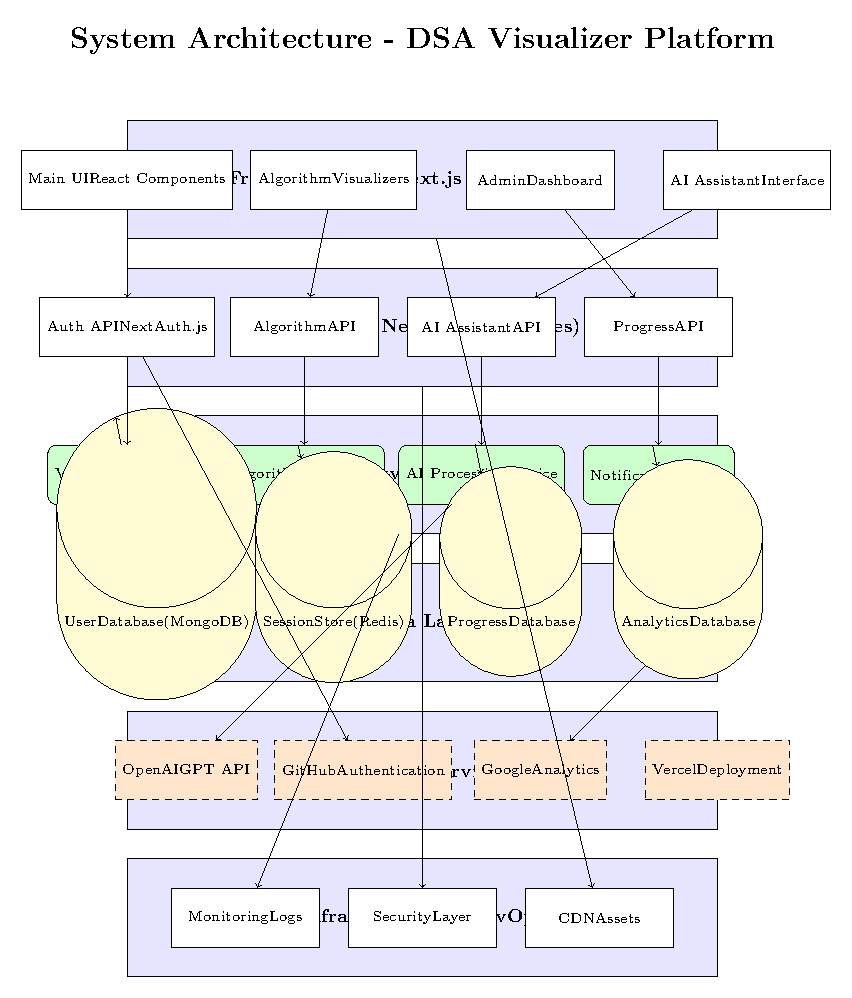
\includegraphics[width=0.9\textwidth]{diagrams/system_architecture.pdf}
\caption{Kiến trúc tổng thể hệ thống DSA Visualizer}
\label{fig:system_architecture}
\end{figure}

\subsubsection{Presentation Layer (Frontend)}
\begin{itemize}
    \item \textbf{Next.js 15 App Router}: Framework chính với server-side rendering
    \item \textbf{React 19}: UI library với concurrent features và hooks mới
    \item \textbf{TypeScript}: Type safety và developer experience
    \item \textbf{Tailwind CSS + shadcn/ui}: Modern styling với component library
    \item \textbf{Framer Motion}: Animation library cho smooth transitions
\end{itemize}

\subsubsection{Business Logic Layer}
\begin{itemize}
    \item \textbf{Algorithm Engines}: Core logic cho 24+ visualization algorithms
    \item \textbf{AI Integration}: OpenAI GPT và Google Gemini APIs
    \item \textbf{Authentication}: NextAuth.js với multi-provider support
    \item \textbf{State Management}: React Context và custom hooks
\end{itemize}

\subsubsection{Data Access Layer}
\begin{itemize}
    \item \textbf{Prisma ORM}: Type-safe database operations
    \item \textbf{API Routes}: Next.js serverless functions
    \item \textbf{Database}: PostgreSQL với connection pooling
    \item \textbf{Caching}: Redis cho session và API response caching
\end{itemize}

\subsection{Use Case Diagram}

\begin{figure}[H]
\centering
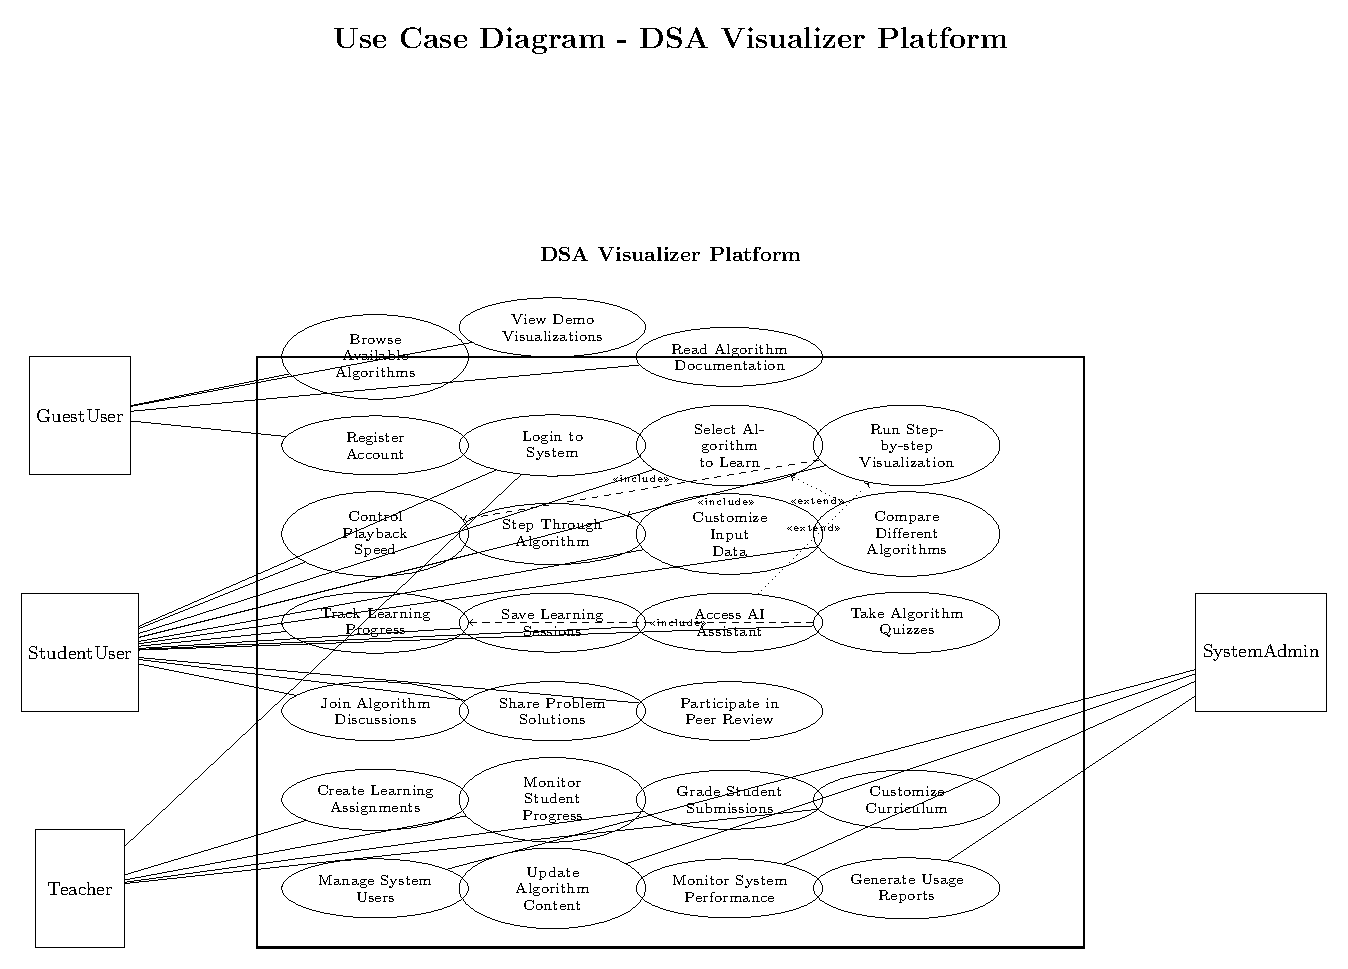
\includegraphics[width=0.9\textwidth]{diagrams/usecase_main.pdf}
\caption{Use Case Diagram - Các chức năng chính của hệ thống}
\label{fig:usecase}
\end{figure}

Use case diagram mô tả các chức năng chính của hệ thống cho từng nhóm người dùng:

\subsubsection{Guest User}
\begin{itemize}
    \item Xem basic algorithm visualizations
    \item Đăng ký tài khoản mới
    \item Truy cập public learning materials
\end{itemize}

\subsubsection{Authenticated User}
\begin{itemize}
    \item Full access đến tất cả visualizers
    \item Sử dụng AI Learning Assistant
    \item Tham gia community forums và Q\&A
    \item Track learning progress
    \item Customize preferences và themes
\end{itemize}

\subsubsection{Teacher}
\begin{itemize}
    \item Tạo và quản lý learning content
    \item Access advanced analytics
    \item Moderate discussions
    \item Create custom algorithm examples
\end{itemize}

\subsubsection{Admin}
\begin{itemize}
    \item User management và role assignment
    \item System monitoring và performance analytics
    \item Content moderation và feedback management
    \item System configuration và maintenance
\end{itemize}

\subsection{Class Diagram}

\begin{figure}[H]
\centering
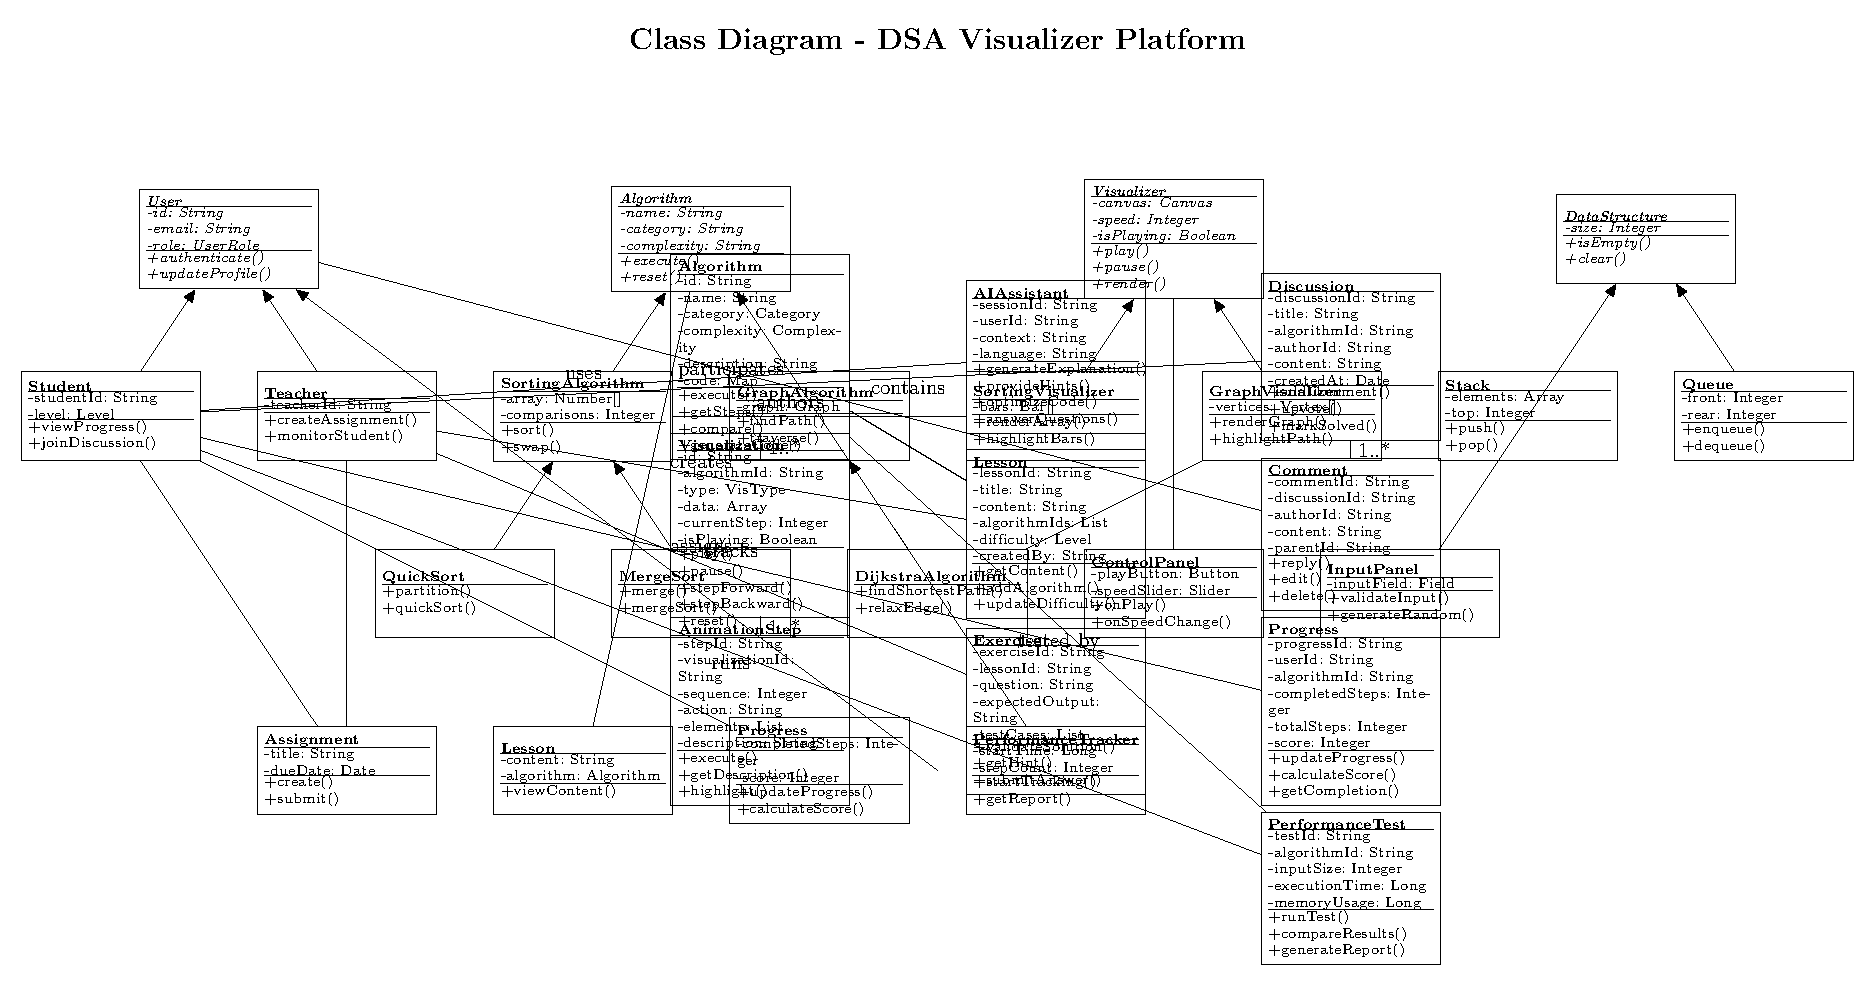
\includegraphics[width=0.9\textwidth]{diagrams/class_diagram.pdf}
\caption{Class Diagram - Cấu trúc lớp chính của hệ thống}
\label{fig:class_diagram}
\end{figure}

Class diagram thể hiện các entities chính và relationships:

\subsubsection{User Management}
\begin{itemize}
    \item \textbf{User}: Base user entity với authentication info
    \item \textbf{Profile}: Extended user information và preferences
    \item \textbf{Role}: Role-based access control system
    \item \textbf{Session}: User session management
\end{itemize}

\subsubsection{Learning System}
\begin{itemize}
    \item \textbf{Algorithm}: Metadata về các thuật toán
    \item \textbf{Visualization}: Visualization instances và state
    \item \textbf{Progress}: User learning progress tracking
    \item \textbf{Tutorial}: Step-by-step learning content
\end{itemize}

\subsubsection{Community Features}
\begin{itemize}
    \item \textbf{Discussion}: Forum discussions và threads
    \item \textbf{Question}: Q\&A system entries
    \item \textbf{Answer}: Responses đến questions
    \item \textbf{Vote}: Voting system cho quality control
\end{itemize}

\subsubsection{Admin System}
\begin{itemize}
    \item \textbf{Analytics}: Usage statistics và metrics
    \item \textbf{Feedback}: User feedback và bug reports
    \item \textbf{SystemConfig}: System-wide configuration
\end{itemize}

\section{Phân tích thiết kế chi tiết}

\subsection{Activity Diagram}

\begin{figure}[H]
\centering
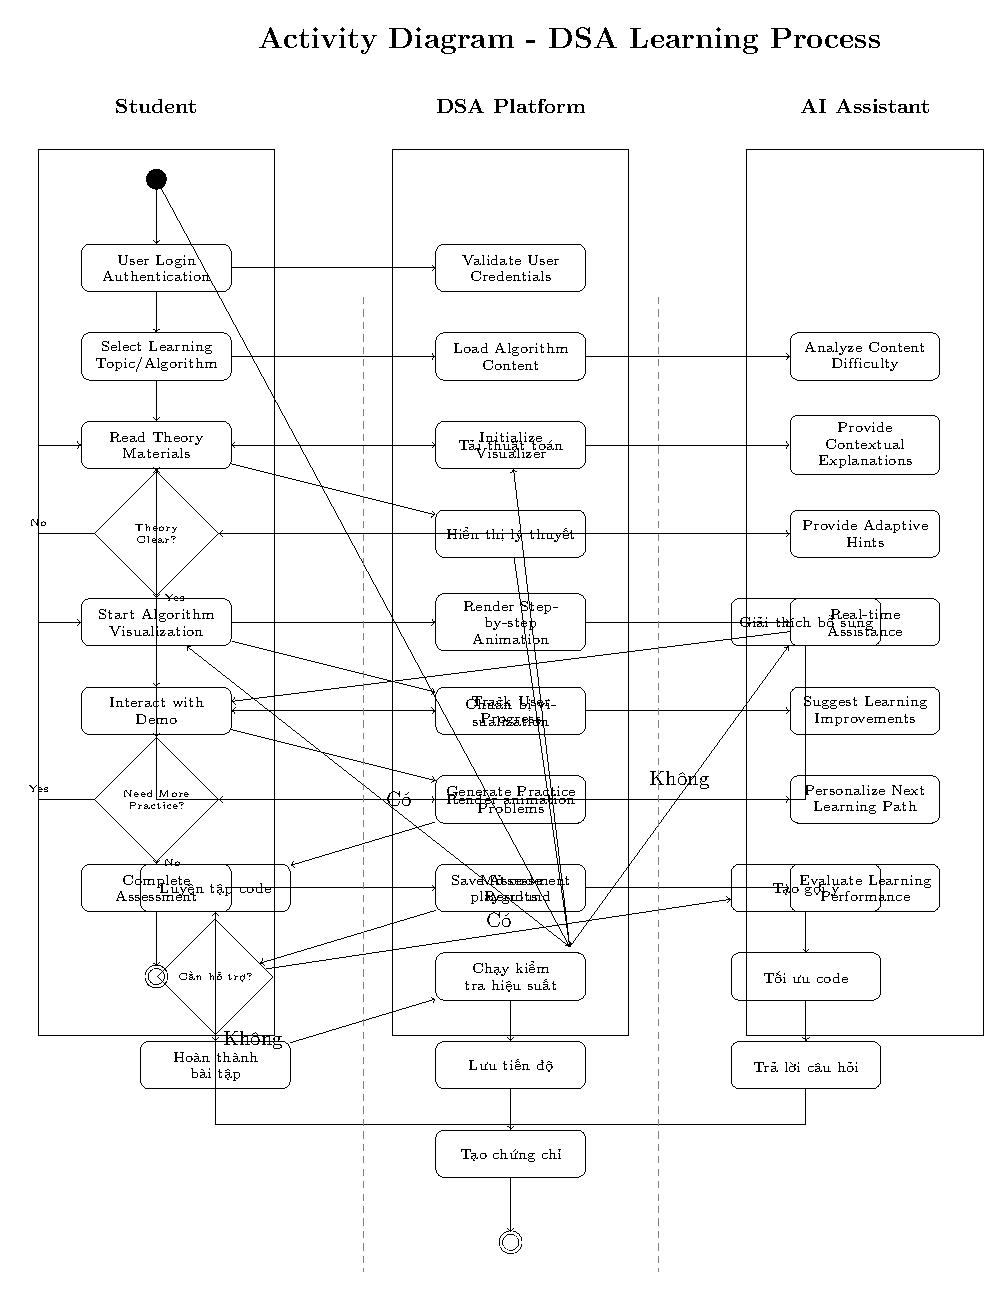
\includegraphics[width=0.9\textwidth]{diagrams/activity_diagram.pdf}
\caption{Activity Diagram - Quy trình học tập với AI assistance}
\label{fig:activity_diagram}
\end{figure}

Activity diagram mô tả quy trình học tập chính của user:

\subsubsection{Giai đoạn khởi tạo}
\begin{enumerate}
    \item User truy cập platform
    \item Hệ thống check authentication status
    \item Load user preferences và progress
    \item Initialize visualization environment
\end{enumerate}

\subsubsection{Giai đoạn chọn thuật toán}
\begin{enumerate}
    \item Browse algorithm categories
    \item Select specific algorithm
    \item Load visualization component
    \item Display algorithm information
\end{enumerate}

\subsubsection{Giai đoạn visualization}
\begin{enumerate}
    \item Configure input parameters
    \item Start algorithm execution
    \item Display step-by-step animation
    \item Provide real-time explanations
    \item Track user interactions
\end{enumerate}

\subsubsection{Giai đoạn AI assistance}
\begin{enumerate}
    \item User requests help hoặc explanation
    \item AI analyzes current context
    \item Generate personalized response
    \item Display interactive code examples
    \item Update learning progress
\end{enumerate}

\subsection{Sequence Diagram}

\begin{figure}[H]
\centering
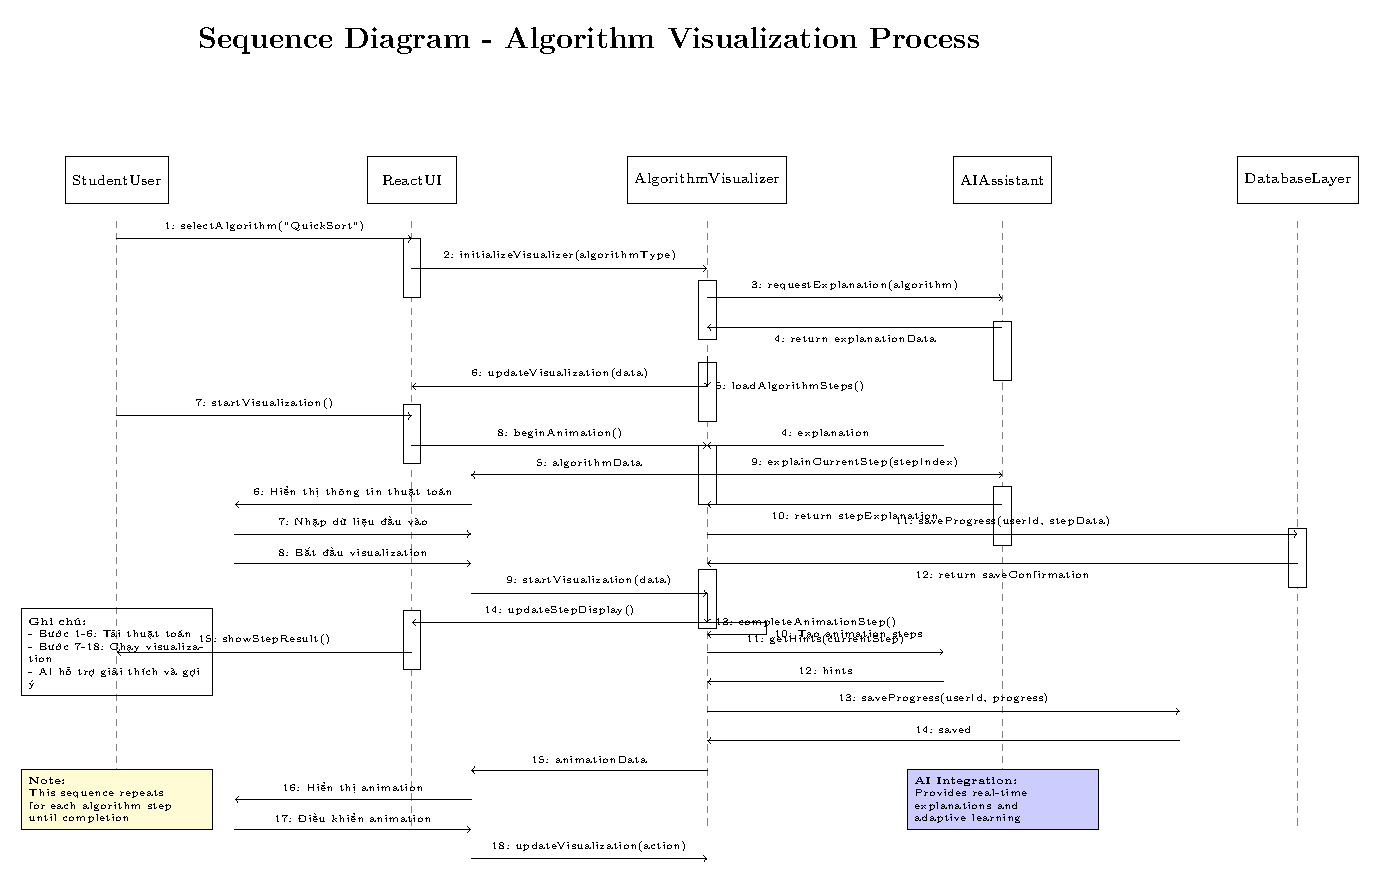
\includegraphics[width=0.9\textwidth]{diagrams/sequence_diagram.pdf}
\caption{Sequence Diagram - Tương tác giữa các components chính}
\label{fig:sequence_diagram}
\end{figure}

Sequence diagram mô tả tương tác giữa các thành phần trong quá trình visualization:

\subsubsection{Khởi tạo visualization}
\begin{enumerate}
    \item \textbf{User Interface} → \textbf{Algorithm Controller}: Request algorithm execution
    \item \textbf{Algorithm Controller} → \textbf{Algorithm Engine}: Initialize algorithm với input data
    \item \textbf{Algorithm Engine} → \textbf{Step Generator}: Generate step-by-step execution plan
    \item \textbf{Step Generator} → \textbf{Animation Controller}: Prepare animation sequences
\end{enumerate}

\subsubsection{Execution và rendering}
\begin{enumerate}
    \item \textbf{Animation Controller} → \textbf{Renderer}: Start animation loop
    \item \textbf{Renderer} → \textbf{UI Components}: Update visual elements
    \item \textbf{UI Components} → \textbf{User Interface}: Display current state
    \item \textbf{Algorithm Engine} → \textbf{Progress Tracker}: Update completion status
\end{enumerate}

\subsubsection{AI interaction}
\begin{enumerate}
    \item \textbf{User Interface} → \textbf{AI Assistant}: Request explanation
    \item \textbf{AI Assistant} → \textbf{AI API}: Send context và query
    \item \textbf{AI API} → \textbf{AI Assistant}: Return generated response
    \item \textbf{AI Assistant} → \textbf{User Interface}: Display explanation
\end{enumerate}
    \item \textbf{Quản trị viên}: Người quản lý nội dung, người dùng và phân tích hệ thống
    \item \textbf{Cộng đồng học tập}: Nhóm người dùng tham gia thảo luận và chia sẻ kiến thức
\end{itemize}

\subsection{Yêu cầu chức năng và phi chức năng}

\subsubsection{Yêu cầu chức năng}
\begin{enumerate}
    \item \textbf{Đối với Học sinh/Sinh viên:}
    \begin{itemize}
        \item Xem và học lý thuyết thuật toán
        \item Chạy visualization tương tác
        \item Thực hành với Code Playground
        \item Sử dụng AI Assistant để hỗ trợ học tập
        \item Theo dõi tiến độ học tập
        \item Tham gia thảo luận cộng đồng
    \end{itemize}
    
    \item \textbf{Đối với Giảng viên:}
    \begin{itemize}
        \item Tạo và quản lý bài giảng
        \item Giao bài tập cho học sinh
        \item Theo dõi tiến độ học tập của lớp
        \item Chấm điểm và phản hồi
        \item Tạo chương trình khuyến mãi
        \item Báo cáo và thống kê
    \end{itemize}
\end{enumerate}

\subsubsection{Yêu cầu phi chức năng}
\begin{itemize}
    \item \textbf{Hiệu suất}: Thời gian phản hồi < 3 giây
    \item \textbf{Bảo mật}: Mã hóa dữ liệu nhạy cảm, xác thực người dùng
    \item \textbf{Khả năng mở rộng}: Hỗ trợ tối thiểu 1000 người dùng đồng thời
    \item \textbf{Tính khả dụng}: Uptime ≥ 99.5\%
\end{itemize}

\newpage
\section{Phân tích hệ thống}

\subsection{Use Case Diagram}

Use Case Diagram mô tả các chức năng chính của hệ thống và mối quan hệ giữa các actor với các use case.

\begin{figure}[H]
    \centering
    \documentclass[tikz,border=10pt]{standalone}
\usepackage[utf8]{inputenc}
\usepackage[T1]{fontenc}
\usepackage[vietnamese]{babel}
\usepackage{tikz}
\usetikzlibrary{shapes.geometric, arrows, positioning, shapes.multipart, fit}

\tikzset{
    actor/.style={
        draw,
        shape=rectangle,
        minimum width=1.5cm,
        minimum height=2cm,
        text centered,
        font=\small
    },
    usecase/.style={
        draw,
        ellipse,
        minimum width=2.5cm,
        minimum height=1cm,
        text centered,
        font=\scriptsize,
        text width=2cm,
        align=center
    },
    system/.style={
        draw,
        rectangle,
        minimum width=14cm,
        minimum height=10cm,
        thick
    },
    include/.style={
        draw,
        dashed,
        ->,
        font=\tiny
    },
    extend/.style={
        draw,
        dotted,
        ->,
        font=\tiny
    },
    association/.style={
        draw,
        -
    }
}

\begin{document}
\begin{tikzpicture}[node distance=2.5cm]

% Title
\node[above] at (0,12) {\Large \textbf{Use Case Diagram - DSA Visualizer Platform}};

% ===== ACTORS =====
\node[actor] (guest) at (-10,6) {Guest\\User};
\node[actor] (student) at (-10,2) {Student\\User};
\node[actor] (teacher) at (-10,-2) {Teacher};
\node[actor] (admin) at (10,2) {System\\Admin};

% ===== SYSTEM BOUNDARY =====
\node[system] (system) at (0,2) {};
\node[above] at (0,8.5) {\textbf{DSA Visualizer Platform}};

% ===== GUEST USER USE CASES =====
\node[usecase] (browse_algorithms) at (-5,7) {Browse Available\\Algorithms};
\node[usecase] (view_demos) at (-2,7.5) {View Demo\\Visualizations};
\node[usecase] (read_documentation) at (1,7) {Read Algorithm\\Documentation};

% ===== CORE LEARNING USE CASES =====
\node[usecase] (register_account) at (-5,5.5) {Register\\Account};
\node[usecase] (login_system) at (-2,5.5) {Login to\\System};
\node[usecase] (select_algorithm) at (1,5.5) {Select Algorithm\\to Learn};
\node[usecase] (run_visualization) at (4,5.5) {Run Step-by-step\\Visualization};

% ===== INTERACTIVE FEATURES =====
\node[usecase] (control_playback) at (-5,4) {Control Playback\\Speed};
\node[usecase] (step_through) at (-2,4) {Step Through\\Algorithm};
\node[usecase] (customize_input) at (1,4) {Customize Input\\Data};
\node[usecase] (compare_algorithms) at (4,4) {Compare Different\\Algorithms};

% ===== LEARNING MANAGEMENT =====
\node[usecase] (track_progress) at (-5,2.5) {Track Learning\\Progress};
\node[usecase] (save_sessions) at (-2,2.5) {Save Learning\\Sessions};
\node[usecase] (access_ai_help) at (1,2.5) {Access AI\\Assistant};
\node[usecase] (take_quizzes) at (4,2.5) {Take Algorithm\\Quizzes};

% ===== COLLABORATION FEATURES =====
\node[usecase] (join_discussions) at (-5,1) {Join Algorithm\\Discussions};
\node[usecase] (share_solutions) at (-2,1) {Share Problem\\Solutions};
\node[usecase] (peer_review) at (1,1) {Participate in\\Peer Review};

% ===== TEACHER USE CASES =====
\node[usecase] (create_assignments) at (-5,-0.5) {Create Learning\\Assignments};
\node[usecase] (monitor_students) at (-2,-0.5) {Monitor Student\\Progress};
\node[usecase] (grade_submissions) at (1,-0.5) {Grade Student\\Submissions};
\node[usecase] (customize_curriculum) at (4,-0.5) {Customize\\Curriculum};

% ===== ADMIN USE CASES =====
\node[usecase] (manage_users) at (-5,-2) {Manage System\\Users};
\node[usecase] (update_content) at (-2,-2) {Update Algorithm\\Content};
\node[usecase] (monitor_system) at (1,-2) {Monitor System\\Performance};
\node[usecase] (generate_reports) at (4,-2) {Generate Usage\\Reports};

% ===== ASSOCIATIONS =====
% Guest User associations
\draw[association] (guest) -- (browse_algorithms);
\draw[association] (guest) -- (view_demos);
\draw[association] (guest) -- (read_documentation);
\draw[association] (guest) -- (register_account);

% Student User associations (inherits from guest)
\draw[association] (student) -- (login_system);
\draw[association] (student) -- (select_algorithm);
\draw[association] (student) -- (run_visualization);
\draw[association] (student) -- (control_playback);
\draw[association] (student) -- (step_through);
\draw[association] (student) -- (customize_input);
\draw[association] (student) -- (compare_algorithms);
\draw[association] (student) -- (track_progress);
\draw[association] (student) -- (save_sessions);
\draw[association] (student) -- (access_ai_help);
\draw[association] (student) -- (take_quizzes);
\draw[association] (student) -- (join_discussions);
\draw[association] (student) -- (share_solutions);
\draw[association] (student) -- (peer_review);

% Teacher associations
\draw[association] (teacher) -- (login_system);
\draw[association] (teacher) -- (create_assignments);
\draw[association] (teacher) -- (monitor_students);
\draw[association] (teacher) -- (grade_submissions);
\draw[association] (teacher) -- (customize_curriculum);

% Admin associations
\draw[association] (admin) -- (manage_users);
\draw[association] (admin) -- (update_content);
\draw[association] (admin) -- (monitor_system);
\draw[association] (admin) -- (generate_reports);

% ===== INCLUDE RELATIONSHIPS =====
\draw[include] (run_visualization) -- (control_playback) node[midway,above,font=\tiny] {<<include>>};
\draw[include] (run_visualization) -- (step_through) node[midway,below,font=\tiny] {<<include>>};
\draw[include] (take_quizzes) -- (track_progress) node[midway,right,font=\tiny] {<<include>>};

% ===== EXTEND RELATIONSHIPS =====
\draw[extend] (access_ai_help) -- (run_visualization) node[midway,above,font=\tiny] {<<extend>>};
\draw[extend] (compare_algorithms) -- (select_algorithm) node[midway,below,font=\tiny] {<<extend>>};

\end{tikzpicture}
\end{document}

    \caption{Use Case Diagram tổng quan của hệ thống}
    \label{fig:usecase_main}
\end{figure}

Hệ thống bao gồm 4 actor chính:
\begin{itemize}
    \item \textbf{Khách hàng cá nhân}: Sử dụng các chức năng tìm kiếm, đặt chỗ và quản lý booking
    \item \textbf{Công ty du lịch}: Quản lý tour và khách hàng
    \item \textbf{Đối tác dịch vụ}: Cung cấp các dịch vụ bổ sung
    \item \textbf{Nhân viên công ty}: Hỗ trợ vận hành hệ thống
\end{itemize}

\subsection{Class Diagram}

Class Diagram mô tả cấu trúc của hệ thống thông qua các lớp đối tượng và mối quan hệ giữa chúng.

\begin{figure}[H]
    \centering
    \documentclass[tikz,border=10pt]{standalone}
\usepackage[utf8]{inputenc}
\usepackage[T1]{fontenc}
\usepackage[vietnamese]{babel}
\usepackage{tikz}
\usetikzlibrary{shapes.geometric, arrows, positioning, shapes.multipart, fit, calc}

\tikzset{
    class/.style={
        draw,
        rectangle,
        minimum width=3cm,
        minimum height=1.5cm,
        text centered,
        font=\scriptsize,
        text width=2.8cm,
        align=left
    },
    abstract/.style={
        class,
        font=\scriptsize\itshape
    },
    interface/.style={
        class,
        dashed
    },
    inheritance/.style={
        draw,
        ->,
        -triangle 45
    },
    association/.style={
        draw,
        -
    },
    aggregation/.style={
        draw,
        -,
        diamond
    },
    composition/.style={
        draw,
        -,
        fill=black,
        diamond
    }
}

\begin{document}
\begin{tikzpicture}[node distance=3cm, auto]

% Title
\node[above] at (0,12) {\Large \textbf{Class Diagram - DSA Visualizer Platform}};

% ===== ROW 1: CORE CLASSES =====
% User Management (Top Left)
\node[abstract] (user) at (-12,9) {
    \textbf{User}\\
    \hrule
    -id: String\\
    -email: String\\
    -role: UserRole\\
    \hrule
    +authenticate()\\
    +updateProfile()
};

% Algorithm Base (Top Center)
\node[abstract] (algorithm) at (-4,9) {
    \textbf{Algorithm}\\
    \hrule
    -name: String\\
    -category: String\\
    -complexity: String\\
    \hrule
    +execute()\\
    +reset()
};

% Visualizer Base (Top Right)
\node[abstract] (visualizer) at (4,9) {
    \textbf{Visualizer}\\
    \hrule
    -canvas: Canvas\\
    -speed: Integer\\
    -isPlaying: Boolean\\
    \hrule
    +play()\\
    +pause()\\
    +render()
};

% Data Structure Base (Far Right)
\node[abstract] (datastructure) at (12,9) {
    \textbf{DataStructure}\\
    \hrule
    -size: Integer\\
    \hrule
    +isEmpty()\\
    +clear()
};

% ===== ROW 2: USER IMPLEMENTATIONS =====
\node[class] (student) at (-14,6) {
    \textbf{Student}\\
    \hrule
    -studentId: String\\
    -level: Level\\
    \hrule
    +viewProgress()\\
    +joinDiscussion()
};

\node[class] (teacher) at (-10,6) {
    \textbf{Teacher}\\
    \hrule
    -teacherId: String\\
    \hrule
    +createAssignment()\\
    +monitorStudent()
};

% ===== ROW 2: ALGORITHM IMPLEMENTATIONS =====
\node[class] (sorting) at (-6,6) {
    \textbf{SortingAlgorithm}\\
    \hrule
    -array: Number[]\\
    -comparisons: Integer\\
    \hrule
    +sort()\\
    +swap()
};

\node[class] (graph) at (-2,6) {
    \textbf{GraphAlgorithm}\\
    \hrule
    -graph: Graph\\
    \hrule
    +findPath()\\
    +traverse()
};

% ===== ROW 2: VISUALIZER IMPLEMENTATIONS =====
\node[class] (sortvis) at (2,6) {
    \textbf{SortingVisualizer}\\
    \hrule
    -bars: Bar[]\\
    \hrule
    +renderArray()\\
    +highlightBars()
};

\node[class] (graphvis) at (6,6) {
    \textbf{GraphVisualizer}\\
    \hrule
    -vertices: Vertex[]\\
    \hrule
    +renderGraph()\\
    +highlightPath()
};

% ===== ROW 2: DATA STRUCTURE IMPLEMENTATIONS =====
\node[class] (stack) at (10,6) {
    \textbf{Stack}\\
    \hrule
    -elements: Array\\
    -top: Integer\\
    \hrule
    +push()\\
    +pop()
};

\node[class] (queue) at (14,6) {
    \textbf{Queue}\\
    \hrule
    -front: Integer\\
    -rear: Integer\\
    \hrule
    +enqueue()\\
    +dequeue()
};

% ===== ROW 3: SPECIFIC ALGORITHMS =====
\node[class] (quicksort) at (-8,3) {
    \textbf{QuickSort}\\
    \hrule
    +partition()\\
    +quickSort()
};

\node[class] (mergesort) at (-4,3) {
    \textbf{MergeSort}\\
    \hrule
    +merge()\\
    +mergeSort()
};

\node[class] (dijkstra) at (0,3) {
    \textbf{DijkstraAlgorithm}\\
    \hrule
    +findShortestPath()\\
    +relaxEdge()
};

% ===== ROW 3: UI COMPONENTS =====
\node[class] (controlpanel) at (4,3) {
    \textbf{ControlPanel}\\
    \hrule
    -playButton: Button\\
    -speedSlider: Slider\\
    \hrule
    +onPlay()\\
    +onSpeedChange()
};

\node[class] (inputpanel) at (8,3) {
    \textbf{InputPanel}\\
    \hrule
    -inputField: Field\\
    \hrule
    +validateInput()\\
    +generateRandom()
};

% ===== ROW 4: SUPPORTING CLASSES =====
\node[class] (assignment) at (-10,0) {
    \textbf{Assignment}\\
    \hrule
    -title: String\\
    -dueDate: Date\\
    \hrule
    +create()\\
    +submit()
};

\node[class] (lesson) at (-6,0) {
    \textbf{Lesson}\\
    \hrule
    -content: String\\
    -algorithm: Algorithm\\
    \hrule
    +viewContent()
};

\node[class] (progress) at (-2,0) {
    \textbf{Progress}\\
    \hrule
    -completedSteps: Integer\\
    -score: Integer\\
    \hrule
    +updateProgress()\\
    +calculateScore()
};

\node[class] (performance) at (2,0) {
    \textbf{PerformanceTracker}\\
    \hrule
    -startTime: Long\\
    -stepCount: Integer\\
    \hrule
    +startTracking()\\
    +getReport()
};

% ===== INHERITANCE RELATIONSHIPS =====
% User inheritance
\draw[inheritance] (student) -- (user);
\draw[inheritance] (teacher) -- (user);

% Algorithm inheritance
\draw[inheritance] (sorting) -- (algorithm);
\draw[inheritance] (graph) -- (algorithm);
\draw[inheritance] (quicksort) -- (sorting);
\draw[inheritance] (mergesort) -- (sorting);
\draw[inheritance] (dijkstra) -- (graph);

% Visualizer inheritance
\draw[inheritance] (sortvis) -- (visualizer);
\draw[inheritance] (graphvis) -- (visualizer);

% Data structure inheritance
\draw[inheritance] (stack) -- (datastructure);
\draw[inheritance] (queue) -- (datastructure);

% ===== ASSOCIATION RELATIONSHIPS =====
% Visualizer associations (simplified)
\draw[association] (sortvis) -- (sorting);
\draw[association] (graphvis) -- (dijkstra);

% UI associations
\draw[association] (controlpanel) -- (visualizer);
\draw[association] (inputpanel) -- (datastructure);

% Learning associations
\draw[association] (assignment) -- (student);
\draw[association] (teacher) -- (assignment);
\draw[association] (lesson) -- (algorithm);
\draw[association] (progress) -- (student);
\draw[association] (performance) -- (algorithm);
    -adminId: String\\
    -permissions: List\\
    \hrule
    +manageUsers()\\
    +systemAnalytics()\\
    +manageContent()\\
    +configureSystem()
};

% Algorithm Management Classes
\node[class] (algorithm) at (-3,7) {
    \textbf{Algorithm}\\
    \hrule
    -id: String\\
    -name: String\\
    -category: Category\\
    -complexity: Complexity\\
    -description: String\\
    -code: Map\\
    \hrule
    +execute()\\
    +getSteps()\\
    +compare()\\
    +generateCode()
};

\node[class] (visualization) at (-3,4) {
    \textbf{Visualization}\\
    \hrule
    -id: String\\
    -algorithmId: String\\
    -type: VisType\\
    -data: Array\\
    -currentStep: Integer\\
    -isPlaying: Boolean\\
    \hrule
    +play()\\
    +pause()\\
    +stepForward()\\
    +stepBackward()\\
    +reset()
};

\node[class] (animationStep) at (-3,1) {
    \textbf{AnimationStep}\\
    \hrule
    -stepId: String\\
    -visualizationId: String\\
    -sequence: Integer\\
    -action: String\\
    -elements: List\\
    -description: String\\
    \hrule
    +execute()\\
    +getDescription()\\
    +highlight()
};

% Learning System Classes
\node[class] (aiAssistant) at (2,7) {
    \textbf{AIAssistant}\\
    \hrule
    -sessionId: String\\
    -userId: String\\
    -context: String\\
    -language: String\\
    \hrule
    +generateExplanation()\\
    +provideHints()\\
    +optimizeCode()\\
    +answerQuestions()
};

\node[class] (lesson) at (2,4) {
    \textbf{Lesson}\\
    \hrule
    -lessonId: String\\
    -title: String\\
    -content: String\\
    -algorithmIds: List\\
    -difficulty: Level\\
    -createdBy: String\\
    \hrule
    +getContent()\\
    +addAlgorithm()\\
    +updateDifficulty()
};

\node[class] (exercise) at (2,1) {
    \textbf{Exercise}\\
    \hrule
    -exerciseId: String\\
    -lessonId: String\\
    -question: String\\
    -expectedOutput: String\\
    -testCases: List\\
    \hrule
    +validateSolution()\\
    +getHint()\\
    +submitAnswer()
};

% Community Classes
\node[class] (discussion) at (7,7) {
    \textbf{Discussion}\\
    \hrule
    -discussionId: String\\
    -title: String\\
    -algorithmId: String\\
    -authorId: String\\
    -content: String\\
    -createdAt: Date\\
    \hrule
    +addComment()\\
    +upvote()\\
    +markSolved()
};

\node[class] (comment) at (7,4) {
    \textbf{Comment}\\
    \hrule
    -commentId: String\\
    -discussionId: String\\
    -authorId: String\\
    -content: String\\
    -parentId: String\\
    \hrule
    +reply()\\
    +edit()\\
    +delete()
};

\node[class] (progress) at (7,1) {
    \textbf{Progress}\\
    \hrule
    -progressId: String\\
    -userId: String\\
    -algorithmId: String\\
    -completedSteps: Integer\\
    -totalSteps: Integer\\
    -score: Integer\\
    \hrule
    +updateProgress()\\
    +calculateScore()\\
    +getCompletion()
};

% Performance Classes
\node[class] (performanceTest) at (7,-2) {
    \textbf{PerformanceTest}\\
    \hrule
    -testId: String\\
    -algorithmId: String\\
    -inputSize: Integer\\
    -executionTime: Long\\
    -memoryUsage: Long\\
    \hrule
    +runTest()\\
    +compareResults()\\
    +generateReport()
};

% Inheritance relationships
\draw[inheritance] (student) -- (user);
\draw[inheritance] (teacher) -- (user);
\draw[inheritance] (admin) -- (user);

% Core Algorithm relationships
\draw[association] (algorithm) -- (visualization) node[midway,right] {1..*};
\draw[association] (visualization) -- (animationStep) node[midway,right] {1..*};
\draw[composition] (lesson) -- (algorithm) node[midway,above] {contains};

% User interactions
\draw[association] (student) -- (progress) node[midway,above] {tracks};
\draw[association] (student) -- (aiAssistant) node[midway,above] {uses};
\draw[association] (student) -- (discussion) node[midway,above] {participates};

% Teacher relationships
\draw[association] (teacher) -- (lesson) node[midway,above] {creates};
\draw[association] (teacher) -- (exercise) node[midway,above] {assigns};

% Community relationships
\draw[association] (discussion) -- (comment) node[midway,right] {1..*};
\draw[association] (user) -- (comment) node[midway,below] {authors};

% Performance monitoring
\draw[association] (algorithm) -- (performanceTest) node[midway,below] {tested by};
\draw[association] (student) -- (performanceTest) node[midway,below] {runs};

\end{tikzpicture}
\end{document}

    \caption{Class Diagram của hệ thống}
    \label{fig:class_diagram}
\end{figure}

Các lớp chính trong hệ thống:
\begin{itemize}
    \item \textbf{User}: Lớp cơ sở cho Customer và Admin
    \item \textbf{Tour}: Quản lý thông tin tour du lịch
    \item \textbf{Booking}: Xử lý đặt chỗ
    \item \textbf{Payment}: Xử lý thanh toán
    \item \textbf{Service classes}: Flight, Hotel, CarRental, Activity
\end{itemize}

\subsection{Activity Diagram}

Activity Diagram mô tả quy trình nghiệp vụ đặt tour du lịch từ đầu đến cuối.

\begin{figure}[H]
    \centering
    \documentclass[tikz,border=10pt]{standalone}
\usepackage[utf8]{inputenc}
\usepackage[T1]{fontenc}
\usepackage[vietnamese]{babel}
\usepackage{tikz}
\usetikzlibrary{shapes.geometric, arrows, positioning, shapes.multipart, fit}

\tikzset{
    start/.style={
        circle,
        fill=black,
        minimum size=0.3cm
    },
    end/.style={
        circle,
        draw,
        double,
        minimum size=0.3cm
    },
    activity/.style={
        draw,
        rectangle,
        rounded corners,
        minimum width=2.5cm,
        minimum height=0.8cm,
        text centered,
        font=\scriptsize,
        text width=2.3cm,
        align=center
    },
    decision/.style={
        draw,
        diamond,
        minimum width=1.5cm,
        minimum height=1cm,
        text centered,
        font=\tiny,
        text width=1.3cm,
        align=center
    },
    fork/.style={
        draw,
        rectangle,
        fill=black,
        minimum width=3cm,
        minimum height=0.1cm
    },
    swimlane/.style={
        draw,
        rectangle,
        minimum width=4cm,
        minimum height=15cm,
        text centered,
        font=\small
    }
}

\begin{document}
\begin{tikzpicture}[node distance=1.8cm]

% Title
\node[above] at (0,15) {\Large \textbf{Activity Diagram - DSA Learning Process}};

% ===== SWIMLANES =====
\node[swimlane] (student_lane) at (-7,6) {};
\node[above] at (-7,14) {\textbf{Student}};

\node[swimlane] (system_lane) at (-1,6) {};
\node[above] at (-1,14) {\textbf{DSA Platform}};

\node[swimlane] (ai_lane) at (5,6) {};
\node[above] at (5,14) {\textbf{AI Assistant}};

% ===== STUDENT ACTIVITIES =====
\node[start] (start) at (-7,13) {};

\node[activity] (login) at (-7,11.5) {User Login\\Authentication};

\node[activity] (select_topic) at (-7,10) {Select Learning\\Topic/Algorithm};

\node[activity] (read_theory) at (-7,8.5) {Read Theory\\Materials};

\node[decision] (understand_theory) at (-7,7) {Theory\\Clear?};

\node[activity] (start_visualization) at (-7,5.5) {Start Algorithm\\Visualization};

\node[activity] (interact_demo) at (-7,4) {Interact with\\Demo};

\node[decision] (practice_needed) at (-7,2.5) {Need More\\Practice?};

\node[activity] (complete_assessment) at (-7,1) {Complete\\Assessment};

\node[end] (end) at (-7,-0.5) {};

% ===== SYSTEM ACTIVITIES =====
\node[activity] (validate_user) at (-1,11.5) {Validate User\\Credentials};

\node[activity] (load_content) at (-1,10) {Load Algorithm\\Content};

\node[activity] (prepare_visualizer) at (-1,8.5) {Initialize\\Visualizer};

\node[activity] (render_animation) at (-1,5.5) {Render Step-by-step\\Animation};

\node[activity] (track_progress) at (-1,4) {Track User\\Progress};

\node[activity] (generate_practice) at (-1,2.5) {Generate Practice\\Problems};

\node[activity] (save_results) at (-1,1) {Save Assessment\\Results};

% ===== AI ASSISTANT ACTIVITIES =====
\node[activity] (analyze_difficulty) at (5,10) {Analyze Content\\Difficulty};

\node[activity] (provide_explanation) at (5,8.5) {Provide Contextual\\Explanations};

\node[activity] (adaptive_hints) at (5,7) {Provide Adaptive\\Hints};

\node[activity] (real_time_help) at (5,5.5) {Real-time\\Assistance};

\node[activity] (suggest_improvements) at (5,4) {Suggest Learning\\Improvements};

\node[activity] (personalize_content) at (5,2.5) {Personalize Next\\Learning Path};

\node[activity] (evaluate_performance) at (5,1) {Evaluate Learning\\Performance};

% ===== FLOW CONNECTIONS =====
% Main student flow
\draw[->] (start) -- (login);
\draw[->] (login) -- (select_topic);
\draw[->] (select_topic) -- (read_theory);
\draw[->] (read_theory) -- (understand_theory);
\draw[->] (understand_theory) -- node[right,font=\tiny] {Yes} (start_visualization);
\draw[->] (start_visualization) -- (interact_demo);
\draw[->] (interact_demo) -- (practice_needed);
\draw[->] (practice_needed) -- node[right,font=\tiny] {No} (complete_assessment);
\draw[->] (complete_assessment) -- (end);

% Loop back connections
\draw[->] (understand_theory) -| node[above,font=\tiny] {No} (-9,7) |- (read_theory);
\draw[->] (practice_needed) -| node[above,font=\tiny] {Yes} (-9,2.5) |- (start_visualization);

% System interactions
\draw[->] (login) -- (validate_user);
\draw[->] (select_topic) -- (load_content);
\draw[->] (read_theory) -- (prepare_visualizer);
\draw[->] (start_visualization) -- (render_animation);
\draw[->] (interact_demo) -- (track_progress);
\draw[->] (practice_needed) -- (generate_practice);
\draw[->] (complete_assessment) -- (save_results);

% AI interactions
\draw[->] (load_content) -- (analyze_difficulty);
\draw[->] (prepare_visualizer) -- (provide_explanation);
\draw[->] (understand_theory) -- (adaptive_hints);
\draw[->] (render_animation) -- (real_time_help);
\draw[->] (track_progress) -- (suggest_improvements);
\draw[->] (generate_practice) -- (personalize_content);
\draw[->] (save_results) -- (evaluate_performance);

% Cross-lane feedback
\draw[->] (adaptive_hints) -- (understand_theory);
\draw[->] (real_time_help) -- (interact_demo);
\draw[->] (personalize_content) -- (practice_needed);
\node[activity] (practice_code) at (-6,1) {Luyện tập code};
\node[decision] (need_help) at (-6,-0.5) {Cần hỗ trợ?};
\node[activity] (complete_exercise) at (-6,-2) {Hoàn thành bài tập};

% Activities in System lane
\node[activity] (load_algorithm) at (-1,8.5) {Tải thuật toán};
\node[activity] (display_theory) at (-1,7) {Hiển thị lý thuyết};
\node[activity] (prepare_visualization) at (-1,4) {Chuẩn bị visualization};
\node[activity] (render_animation) at (-1,2.5) {Render animation};
\node[activity] (code_playground) at (-1,1) {Mở code playground};
\node[activity] (run_performance_test) at (-1,-0.5) {Chạy kiểm tra hiệu suất};
\node[activity] (save_progress) at (-1,-2) {Lưu tiến độ};
\node[activity] (generate_certificate) at (-1,-3.5) {Tạo chứng chỉ};

% Activities in AI lane
\node[activity] (provide_explanation) at (4,5.5) {Giải thích bổ sung};
\node[activity] (generate_hints) at (4,1) {Tạo gợi ý};
\node[activity] (optimize_code) at (4,-0.5) {Tối ưu code};
\node[activity] (answer_questions) at (4,-2) {Trả lời câu hỏi};

% End states
\node[end] (end_success) at (-1,-5) {};

% Main flow arrows
\draw[->] (start) -- (select_algorithm);
\draw[->] (select_algorithm) -- (load_algorithm);
\draw[->] (load_algorithm) -- (read_theory);
\draw[->] (read_theory) -- (display_theory);
\draw[->] (display_theory) -- (understand);

% Understanding decision
\draw[->] (understand) -- (start_visualization) node[midway,right] {Có};
\draw[->] (understand) -- (provide_explanation) node[midway,above] {Không};
\draw[->] (provide_explanation) -- ++(0,-3) -| (read_theory);

\draw[->] (start_visualization) -- (prepare_visualization);
\draw[->] (prepare_visualization) -- (interact_demo);
\draw[->] (interact_demo) -- (render_animation);
\draw[->] (render_animation) -- (practice_code);
\draw[->] (practice_code) -- (code_playground);
\draw[->] (code_playground) -- (need_help);

% Help decision
\draw[->] (need_help) -- (complete_exercise) node[midway,right] {Không};
\draw[->] (need_help) -- (generate_hints) node[midway,above] {Có};
\draw[->] (generate_hints) -- (optimize_code);
\draw[->] (optimize_code) -- (answer_questions);
\draw[->] (answer_questions) -- ++(0,-1) -| (practice_code);

\draw[->] (complete_exercise) -- (run_performance_test);
\draw[->] (run_performance_test) -- (save_progress);
\draw[->] (save_progress) -- (generate_certificate);
\draw[->] (generate_certificate) -- (end_success);

% Dotted lines for swimlane boundaries
\draw[dashed, gray] (-3.5,11) -- (-3.5,-5.5);
\draw[dashed, gray] (1.5,11) -- (1.5,-5.5);

\end{tikzpicture}
\end{document}


    \caption{Activity Diagram - Quy trình đặt tour}
    \label{fig:activity_diagram}
\end{figure}

Quy trình bao gồm các bước chính:
\begin{enumerate}
    \item Tìm kiếm tour
    \item Chọn và xem chi tiết
    \item Nhập thông tin đặt chỗ
    \item Xử lý thanh toán
    \item Xác nhận booking
\end{enumerate}

\subsection{Sequence Diagram}

Sequence Diagram mô tả tương tác giữa các đối tượng trong quá trình đặt tour theo thời gian.

\begin{figure}[H]
    \centering
    \documentclass[tikz,border=10pt]{standalone}
\usepackage[utf8]{inputenc}
\usepackage[T1]{fontenc}
\usepackage[vietnamese]{babel}
\usepackage{tikz}
\usetikzlibrary{shapes.geometric, arrows, positioning, shapes.multipart, fit, calc}

\tikzset{
    actor/.style={
        draw,
        rectangle,
        minimum width=1.5cm,
        minimum height=0.8cm,
        text centered,
        font=\scriptsize
    },
    lifeline/.style={
        draw,
        dashed,
        gray
    },
    message/.style={
        draw,
        ->,
        font=\tiny
    },
    selfmessage/.style={
        draw,
        ->,
        font=\tiny
    },
    activation/.style={
        draw,
        rectangle,
        fill=white,
        minimum width=0.3cm,
        minimum height=1cm
    }
}

\begin{document}
\begin{tikzpicture}[node distance=4cm]

% Title
\node[above] at (0,12) {\Large \textbf{Sequence Diagram - Algorithm Visualization Process}};

% ===== ACTORS AND OBJECTS =====
\node[actor] (student) at (-8,10) {Student\\User};
\node[actor] (ui) at (-3,10) {React\\UI};
\node[actor] (visualizer) at (2,10) {Algorithm\\Visualizer};
\node[actor] (ai) at (7,10) {AI\\Assistant};
\node[actor] (database) at (12,10) {Database\\Layer};

% ===== LIFELINES =====
\draw[lifeline] (-8,9.3) -- (-8,-1);
\draw[lifeline] (-3,9.3) -- (-3,-1);
\draw[lifeline] (2,9.3) -- (2,-1);
\draw[lifeline] (7,9.3) -- (7,-1);
\draw[lifeline] (12,9.3) -- (12,-1);

% ===== ACTIVATION BOXES =====
\node[activation] (act1) at (-3,8.5) {};
\node[activation] (act2) at (2,7.8) {};
\node[activation] (act3) at (7,7.1) {};
\node[activation] (act4) at (2,6.4) {};
\node[activation] (act5) at (-3,5.7) {};
\node[activation] (act6) at (2,5) {};
\node[activation] (act7) at (7,4.3) {};
\node[activation] (act8) at (12,3.6) {};
\node[activation] (act9) at (2,2.9) {};
\node[activation] (act10) at (-3,2.2) {};

% ===== MESSAGE SEQUENCE =====
% 1. Student selects algorithm
\draw[message] (-8,9) -- (-3,9) node[midway,above,font=\tiny] {1: selectAlgorithm("QuickSort")};

% 2. UI initializes visualizer
\draw[message] (-3,8.5) -- (2,8.5) node[midway,above,font=\tiny] {2: initializeVisualizer(algorithmType)};

% 3. Visualizer requests AI explanation
\draw[message] (2,8) -- (7,8) node[midway,above,font=\tiny] {3: requestExplanation(algorithm)};

% 4. AI generates explanation
\draw[message] (7,7.5) -- (2,7.5) node[midway,below,font=\tiny] {4: return explanationData};

% 5. Visualizer loads algorithm
\draw[message] (2,7) -- (2,6.5) node[right,font=\tiny] {5: loadAlgorithmSteps()};

% 6. Visualizer updates UI
\draw[message] (2,6.5) -- (-3,6.5) node[midway,above,font=\tiny] {6: updateVisualization(data)};

% 7. Student starts visualization
\draw[message] (-8,6) -- (-3,6) node[midway,above,font=\tiny] {7: startVisualization()};

% 8. UI starts animation
\draw[message] (-3,5.5) -- (2,5.5) node[midway,above,font=\tiny] {8: beginAnimation()};

% 9. Visualizer asks AI for step explanation
\draw[message] (2,5) -- (7,5) node[midway,above,font=\tiny] {9: explainCurrentStep(stepIndex)};

% 10. AI provides step explanation
\draw[message] (7,4.5) -- (2,4.5) node[midway,below,font=\tiny] {10: return stepExplanation};

% 11. Visualizer saves progress
\draw[message] (2,4) -- (12,4) node[midway,above,font=\tiny] {11: saveProgress(userId, stepData)};

% 12. Database confirms save
\draw[message] (12,3.5) -- (2,3.5) node[midway,below,font=\tiny] {12: return saveConfirmation};

% 13. Visualizer completes step
\draw[message] (2,3) -- (2,2.5) node[right,font=\tiny] {13: completeAnimationStep()};

% 14. UI updates display
\draw[message] (2,2.5) -- (-3,2.5) node[midway,above,font=\tiny] {14: updateStepDisplay()};

% 15. Display result to student
\draw[message] (-3,2) -- (-8,2) node[midway,above,font=\tiny] {15: showStepResult()};

% ===== NOTES =====
\node[draw,rectangle,fill=yellow!20,text width=3cm,font=\tiny] at (-8,-0.5) {
    \textbf{Note:}\\
    This sequence repeats\\
    for each algorithm step\\
    until completion
};

\node[draw,rectangle,fill=blue!20,text width=3cm,font=\tiny] at (7,-0.5) {
    \textbf{AI Integration:}\\
    Provides real-time\\
    explanations and\\
    adaptive learning
};

% 4. AI returns explanation
\draw[message] (6,5.5) -- (2,5.5) node[midway,above] {4: explanation};

% 5. Visualizer returns algorithm data
\draw[message] (2,5) -- (-2,5) node[midway,above] {5: algorithmData};

% 6. UI displays algorithm info
\draw[message] (-2,4.5) -- (-6,4.5) node[midway,above] {6: Hiển thị thông tin thuật toán};

% 7. Student inputs data
\draw[message] (-6,4) -- (-2,4) node[midway,above] {7: Nhập dữ liệu đầu vào};

% 8. Student starts visualization
\draw[message] (-6,3.5) -- (-2,3.5) node[midway,above] {8: Bắt đầu visualization};

% 9. UI starts visualization
\draw[message] (-2,3) -- (2,3) node[midway,above] {9: startVisualization(data)};

% 10. Visualizer generates steps
\draw[selfmessage] (2,2.5) -- ++(1,0) |- (2,2.3) node[midway,right] {10: Tạo animation steps};

% 11. Visualizer gets AI hints
\draw[message] (2,2) -- (6,2) node[midway,above] {11: getHints(currentStep)};

% 12. AI provides hints
\draw[message] (6,1.5) -- (2,1.5) node[midway,above] {12: hints};

% 13. Visualizer saves progress
\draw[message] (2,1) -- (10,1) node[midway,above] {13: saveProgress(userId, progress)};

% 14. Database confirms save
\draw[message] (10,0.5) -- (2,0.5) node[midway,above] {14: saved};

% 15. Visualizer returns animation
\draw[message] (2,0) -- (-2,0) node[midway,above] {15: animationData};

% 16. UI renders visualization
\draw[message] (-2,-0.5) -- (-6,-0.5) node[midway,above] {16: Hiển thị animation};

% 17. Student interacts with controls
\draw[message] (-6,-1) -- (-2,-1) node[midway,above] {17: Điều khiển animation};

% 18. UI updates visualization
\draw[message] (-2,-1.5) -- (2,-1.5) node[midway,above] {18: updateVisualization(action)};

% Notes
\node[draw, rectangle, text width=3cm, font=\tiny] at (-8,2) {
    \textbf{Ghi chú:}\\
    - Bước 1-6: Tải thuật toán\\
    - Bước 7-18: Chạy visualization\\
    - AI hỗ trợ giải thích và gợi ý
};

\end{tikzpicture}
\end{document}


    \caption{Sequence Diagram - Đặt tour du lịch}
    \label{fig:sequence_diagram}
\end{figure}

Tương tác diễn ra giữa:
\begin{itemize}
    \item Khách hàng và Giao diện Web
    \item Giao diện Web và Tour Controller
    \item Tour Controller và Cơ sở dữ liệu
    \item Tour Controller và Hệ thống Thanh toán
\end{itemize}

\newpage
\section{Kiến trúc hệ thống}

\subsection{System Architecture}

Kiến trúc hệ thống được thiết kế theo mô hình phân tầng (Layered Architecture) để đảm bảo tính module, dễ bảo trì và mở rộng.

\begin{figure}[H]
    \centering
    \documentclass[tikz,border=10pt]{standalone}
\usepackage[utf8]{inputenc}
\usepackage[T1]{fontenc}
\usepackage[vietnamese]{babel}
\usepackage{tikz}
\usetikzlibrary{shapes.geometric, arrows, positioning, shapes.multipart, fit, calc}

\tikzset{
    layer/.style={
        draw,
        rectangle,
        minimum width=10cm,
        minimum height=2cm,
        text centered,
        font=\small,
        fill=blue!10
    },
    component/.style={
        draw,
        rectangle,
        minimum width=2.5cm,
        minimum height=1cm,
        text centered,
        font=\scriptsize,
        fill=white
    },
    database/.style={
        draw,
        cylinder,
        shape border rotate=90,
        minimum width=2cm,
        minimum height=1.5cm,
        text centered,
        font=\scriptsize,
        fill=yellow!20
    },
    service/.style={
        draw,
        rectangle,
        rounded corners,
        minimum width=2cm,
        minimum height=1cm,
        text centered,
        font=\scriptsize,
        fill=green!20
    },
    external/.style={
        draw,
        rectangle,
        dashed,
        minimum width=2cm,
        minimum height=1cm,
        text centered,
        font=\scriptsize,
        fill=orange!20
    }
}

\begin{document}
\begin{tikzpicture}[node distance=2.5cm]

% Title
\node[above] at (0,15) {\Large \textbf{System Architecture - DSA Visualizer Platform}};

% ===== PRESENTATION LAYER =====
\node[layer] (presentation) at (0,13) {\textbf{Frontend Layer (Next.js 15 + React 19)}};

% Frontend components with better spacing
\node[component] (main_ui) at (-5,13) {Main UI\\React Components};
\node[component] (visualizers) at (-1.5,13) {Algorithm\\Visualizers};
\node[component] (admin_ui) at (2,13) {Admin\\Dashboard};
\node[component] (ai_chat) at (5.5,13) {AI Assistant\\Interface};

% ===== API LAYER =====
\node[layer] (api_layer) at (0,10.5) {\textbf{API Layer (Next.js API Routes)}};

% API endpoints with proper spacing
\node[component] (auth_api) at (-5,10.5) {Auth API\\NextAuth.js};
\node[component] (algorithm_api) at (-2,10.5) {Algorithm\\API};
\node[component] (ai_api) at (1,10.5) {AI Assistant\\API};
\node[component] (progress_api) at (4,10.5) {Progress\\API};

% ===== SERVICE LAYER =====
\node[layer] (service) at (0,8) {\textbf{Service Layer}};

% Services with better positioning
\node[service] (visualizer_service) at (-5,8) {Visualization\\Engine};
\node[service] (algorithm_service) at (-2,8) {Algorithm\\Execution};
\node[service] (ai_service) at (1,8) {AI Processing\\Service};
\node[service] (notification_service) at (4,8) {Notification\\Service};

% ===== DATA LAYER =====
\node[layer] (data_layer) at (0,5.5) {\textbf{Data Layer}};

% Databases with proper spacing
\node[database] (user_db) at (-4.5,5.5) {User\\Database\\(MongoDB)};
\node[database] (session_db) at (-1.5,5.5) {Session\\Store\\(Redis)};
\node[database] (progress_db) at (1.5,5.5) {Progress\\Database};
\node[database] (analytics_db) at (4.5,5.5) {Analytics\\Database};

% ===== EXTERNAL SERVICES =====
\node[layer] (external_layer) at (0,3) {\textbf{External Services}};

% External services properly spaced
\node[external] (openai) at (-4,3) {OpenAI\\GPT API};
\node[external] (github) at (-1,3) {GitHub\\Authentication};
\node[external] (google) at (2,3) {Google\\Analytics};
\node[external] (vercel) at (5,3) {Vercel\\Deployment};

% ===== INFRASTRUCTURE =====
\node[layer] (infrastructure) at (0,0.5) {\textbf{Infrastructure \& DevOps}};

% Infrastructure components
\node[component] (monitoring) at (-3,0.5) {Monitoring\\Logs};
\node[component] (security) at (0,0.5) {Security\\Layer};
\node[component] (cdn) at (3,0.5) {CDN\\Assets};

% ===== CONNECTIONS =====
% Frontend to API
\draw[->] (main_ui) -- (auth_api);
\draw[->] (visualizers) -- (algorithm_api);
\draw[->] (admin_ui) -- (progress_api);
\draw[->] (ai_chat) -- (ai_api);

% API to Services
\draw[->] (auth_api) -- (visualizer_service);
\draw[->] (algorithm_api) -- (algorithm_service);
\draw[->] (ai_api) -- (ai_service);
\draw[->] (progress_api) -- (notification_service);

% Services to Data
\draw[->] (visualizer_service) -- (user_db);
\draw[->] (algorithm_service) -- (session_db);
\draw[->] (ai_service) -- (progress_db);
\draw[->] (notification_service) -- (analytics_db);

% External connections
\draw[->] (ai_service) -- (openai);
\draw[->] (auth_api) -- (github);
\draw[->] (analytics_db) -- (google);

% Infrastructure connections
\draw[->] (service) -- (monitoring);
\draw[->] (api_layer) -- (security);
\draw[->] (presentation) -- (cdn);

\end{tikzpicture}
\end{document}

    \caption{Kiến trúc tổng thể của hệ thống}
    \label{fig:system_architecture}
\end{figure}

Hệ thống bao gồm các tầng:

\subsubsection{Tầng Giao diện (Presentation Layer)}
\begin{itemize}
    \item \textbf{Web UI}: Giao diện web sử dụng React/Vue.js
    \item \textbf{Mobile UI}: Ứng dụng di động với React Native
    \item \textbf{Admin Panel}: Giao diện quản trị cho nhân viên
\end{itemize}

\subsubsection{Tầng Logic Nghiệp vụ (Business Layer)}
\begin{itemize}
    \item \textbf{Tour Service}: Xử lý logic liên quan đến tour
    \item \textbf{Booking Service}: Quản lý đặt chỗ
    \item \textbf{Payment Service}: Xử lý thanh toán
    \item \textbf{User Service}: Quản lý người dùng
\end{itemize}

\subsubsection{Tầng Truy cập Dữ liệu (Data Access Layer)}
Các DAO (Data Access Object) để tương tác với cơ sở dữ liệu:
\begin{itemize}
    \item Tour DAO, Booking DAO, User DAO, Payment DAO
\end{itemize}

\subsubsection{Tầng Cơ sở Dữ liệu (Database Layer)}
\begin{itemize}
    \item \textbf{PostgreSQL}: Cơ sở dữ liệu chính
    \item \textbf{Redis}: Cache để tăng hiệu suất
    \item \textbf{AWS S3}: Lưu trữ file và hình ảnh
\end{itemize}

\subsubsection{Dịch vụ Bên ngoài (External Services)}
\begin{itemize}
    \item Payment Gateway (Stripe/PayPal)
    \item Email Service (SendGrid)
    \item Maps API (Google Maps)
    \item Weather API
    \item Flight API (Amadeus)
\end{itemize}

\section{Kết luận và Hướng phát triển}

\subsection{Kết luận}
Hệ thống website đặt chỗ và gợi ý địa điểm du lịch đã được thiết kế với kiến trúc phân tầng rõ ràng, đáp ứng đầy đủ các yêu cầu chức năng và phi chức năng. Các diagram UML đã mô tả chi tiết:

\begin{itemize}
    \item Các actor và use case chính của hệ thống
    \item Cấu trúc lớp đối tượng và mối quan hệ
    \item Quy trình nghiệp vụ đặt tour
    \item Tương tác giữa các thành phần theo thời gian
    \item Kiến trúc tổng thể của hệ thống
\end{itemize}

\subsection{Hướng phát triển}
\begin{itemize}
    \item Tích hợp AI để gợi ý tour cá nhân hóa
    \item Phát triển ứng dụng mobile native
    \item Triển khai microservices architecture
    \item Tích hợp thêm các dịch vụ bên thứ ba
    \item Phát triển hệ thống báo cáo và analytics
\end{itemize}

\end{document}
